\chapter{Introduction}
This chapter introduces the concept of an organic radical battery, the electrochemical processes in the battery electrodes, the structures of organic electrode materials based on redox conductive polymers and their electrochemical performance. Necessary electrochemical characterization techniques are described. Charge transport models for particular electro-active conjugated polymers are reviewed.

%\paragraph*{}
%Life needs energy to continue its spread. Plants use photosynthesis to separate carbon from oxygen and to grow. Higher life forms as humans consume energy during the day and during the night, being dependent on the available energy source~\cite{energy_consumption_review}. While fossil fuels are still the major source of energy~\cite{energy_sources_review} and while fire is used to convert the Joules that hold together hydrocarbon molecules into a "horse power" of a combustion engine and kilowatt-hours in a power socket, there are cleaner and more efficient ways to harvest energy. Photosynthesis had inspired the creation of solar panels that convert the sunlight into electricity, the atom had been tamed in the core of a nuclear reactor to power cities; we can extract energy from sound~\cite{energy_from_sound}, wind and waves and from the heat of the planet. Moreover, there are hopes and continuous attempts to achieve nuclear fusion~\cite{tokamak_updates} - the creation of an artificial Sun by melting together atomic cores - the virtually inexhaustible and clean source of energy. The oil and gas are limited and unevenly distributed resources, wind does not always blow, the Sun does not shine at night, the wild Nature is still unpredictable and the extracted energy has to be stored in order to level out its production and consumption.\\
%
%\par
%The concept of clean energy can be divided into three components: harvest and conversion of clean energy, energy storage and management~\cite{Liu2016}.\\
%
%\par
%With the rise of the technological era, over the last century, energy has been delivered to our homes in form of electricity. 

\paragraph*{}
Energy storage systems such as fuel cells, supercapacitors and batteries are crucial elements for powering portable electronics, vehicles, and for balancing a power grid with a renewable energy source~\cite{janoschka2012_advmater}. Stable, capacious and powerful batteries have become of great demand for today's energy driven society~\cite{Yoo2014,Xu2020,Nitta2015}. The capacity of installed battery storage systems is predicted to increase upto 400~GWh by 2030~\cite{Figgener_2020}. The advances in lithium ion technology for rechargeable batteries have enabled energy densities that make it possible to battery-power a wearable Internet-of-things device~\cite{Lee2013,Maddikunta2020}, an airplane~\cite{Kadlec2014} or a house~\cite{Diouf2019,Hirasawa2021}. Still, the application of lithium ion batteries is limited by irreversible processes~\cite{Larsson2017,Fu2015,Zhang2021} that occur upon extreme operating conditions such as high power demand~\cite{Zhang2022,Guan2018} or over-discharge~\cite{Ma2020}. Such degradation processes limit the performance of a battery by lowering its safe operating power, resulting in lower power density and longer charging times. The challenge to overcome these limitations, together with low abundance of Lithium, Cobalt and rare earth metals~\cite{Xu2020,janoschka2012_advmater}, the toxicity of the manufacturing process~\cite{Prazanov2022,Peters2017} and the biohazardous nature of the inorganic electrode materials~\cite{Casado_2021_book} is motivating research and development of advanced, organic-based battery technologies~\cite{Degen2022}. This requires understanding of charge transport and degradation pathways in energy storage materials as well as exploring novel materials such as materials based on organic precursors~\cite{Lu2020,Kim2023}.\\

\section{Rechargeable Electrochemical Cells}
Two opposite electric charges separated from each other can store energy in an electrostatic field. It is possible to accumulate many charges on the plates of a capacitor and store some energy~\cite{He_2022}, but due to the technological difficulties, electrochemical cells are commonly used instead~\cite{Figgener_2020}. An electrochemical cell is an energy storage device and a power source that undergoes a chemical reaction to transfer some electric charge from one of its components to another through an external circuit. 

\begin{figure}[h]
\center
	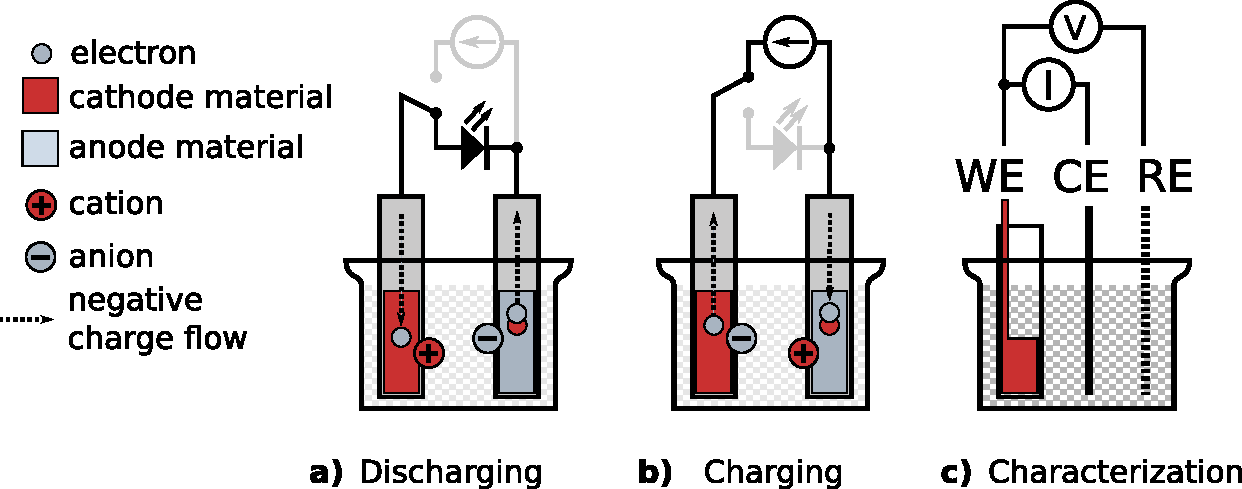
\includegraphics[width=0.95\textwidth]{./electrochemistry/figures/echem_cells.pdf}
	\caption{Rechargeable electrochemical cell connected to an external circuit for discharging a) and charging b). c): Three-electrode half-cell used for electrochemical characterization and charging of the cathode material. d): symbol for an electrochemical cell used in electric diagrams.}
	\label{fig:echem_cells}
\end{figure}

A simple electrochemical cell consists of three elements: two spatially separated materials called electrodes, and a solution of mobile ions between them called electrolyte. The two electrodes have different work functions, or, chemically speaking, reduction-oxidation (redox) potentials. The potential difference between the two electrodes is called the open-circuit potential of the cell, $V_{OC}$. When the electrodes are connected through an external circuit, as shown in Figure~\ref{fig:echem_cells}~a), the charge flows from one electrode to another through the circuit and the ions in the electrolyte rearrange to maintain charge balance~\cite{muench2016_chemrev}. While the cell delivers the electric current to the circuit, a chemical reaction is happening on its electrodes: the positively charged electrode, called cathode, is being reduced, obtaining electrons from the negatively charged anode through the external circuit. At the same time, the anode loses electrons and is being oxidized. If the electrodes can undergo a reversible redox reaction, a current applied to the cell restores its charged state, as shown in Figure~\ref{fig:echem_cells}~b).\\


\subsection{Organic Radical Battery}

Batteries based on redox conductive polymers containing stable radical fragments as high-capacitance groups represent a promising class of future electrochemical power sources - organic radical batteries (ORB)~\cite{nakahara2002_cpl, nishide2004_electact,xie2021_mathoriz,Rohland_2021}. ORB combine the advantages of high-power supercapacitors, namely high discharge rates, and the high energy density of conventional lithium-ion technology. In contrast to the lithium-ion battery, the charging of an organic battery does not involve intercalation of metal ions into the electrodes. This reduces the structural change of the electrode upon repeated recharging which allows for a longer cycle life of ORBs. The electrolyte ions in an ORB do not chemically react with the electrodes, but rearrange to compensate the charges in the electrode, that improves the safety and lifetime of ORBs as compared to the Li technology. The amorphous and swollen structure of organic electrodes allows the electrolyte ions to diffuse into the electrode, which allows for oxidizing or reducing the electrode within its volume - this also increases the charge/discharge rates of ORBs~\cite{nishide_2009}. A further beneficial property of organic materials over traditional inorganic materials is their availability and the low cost of the starting materials for the synthesis of the target polymers in conjunction with good mechanical properties~\cite{janoschka2012_advmater, muench2016_chemrev, friebe2017_topcurrchem}. The large knowledge base on polymer processing allows for inkjet printing, roll-to-roll processing and other low-cost manufacturing techniques for making low-cost, flexible and light-weight integrated devices, including flexible plastic batteries~\cite{janoschka2012_advmater,nishide_2009}. 


\section{Experimental Techniques for Characterizing Battery Materials}
The flexible molecular design together with questions regarding unresolved charge-transport- and performance limiting mechanisms have inspired a variety of characterization techniques to be developed and applied to both energy storage materials and energy storage devices, operando (during the operation of a device) and ex-situ. Together with electrochemical characterization as the standard method for studying the properties of energy storage materials~\cite{Bard_book,IWASA2007,Zens2022}, operando optical microscopy~\cite{Merryweather2022}, neutron imaging~\cite{Ma2020}, mass spectroscopy~\cite{Fang_2021} and X-ray diffraction~\cite{Rhodes2012} were applied to monitor irreversible structural deformations of the components of Li cells during extreme charging conditions.\\

\par UV and IR spectroscopy turned out to be particularly useful for studying organic energy-storage materials. For instance, with UV-Vis spectroscopy, it was possible to observe formation of positive polarons in the conductive molecular backbone for ORBs upon its oxidation~\cite{Dmitrieva2018}.
Since the electrochemical processes happen within the bulk of the energy storage material and involve changes in the spin states, imaging techniques based on magnetic resonance~\cite{Niemoller2018,Meier2013,Li2019,Bittl2005} can be applied to obtain structural information on the battery electrodes at the molecular level. NMR was used to study dendrite formation, electrolyte dynamics and intercalation of Li ions~\cite{Kushida1980,Grosu2023a} in Li cells, including operando imaging~\cite{Shi2019}.\\ 

Operando continuous-wave electron paramagnetic resonance spectroscopy(cwEPR) was applied to study electron transfer rates and electrolyte decomposition in redox-flow batteries~\cite{zhao2021_jacs}, redox kinetics of inorganic battery cathodes~\cite{Niemoller2019}, radical formation and spin densities in redox polymers~\cite{Dmitrieva2018} and in organic electrochemical cells~\cite{huang2016_jpowersources,Kulikov2022,kanzaki2018_acsappmat}.\\

Pulsed EPR (pEPR) provides an even more powerful toolbox for material studies with the electron spin as a microscopic structural probe. In particular, pEPR provides access to the dipolar coupling between neighboring electron spins and thus the possibility to determine distances between adjacent redox-active centers using dipolar spectroscopy~\cite{Salikhov1981} as in spin-labelled proteins~\cite{jeschke2012_annrevphyschem,Toropov1998}. In addition, the hyperfine coupling between electron and nuclear spins in close vicinity can be measured by the electron spin echo envelope modulation (ESEEM) and the electron nuclear double resonance (ENDOR) techniques and can thus elucidate the degree of delocalization for charge carriers in ORB materials in a similar way as in organic seminconductors~\cite{Behrends2011}.\\

However, the high spin concentration in \ik{energy storage materials at certain states of charge (SoC)} implies strong inter-spin interactions \ik{that lead to decoherences between the excited spins}, so the spin echo in \ik{such} dense\ik{ly packed spin system\ik{s}} usually decays much quicker than in the well studied dilute systems such as proteins~\cite{jeschke2012_annrevphyschem} or intrinsic organic semiconductors~\cite{Tait2021}. The quick spin echo decay limits the maximum length of the microwave pulse sequence \rs{and raises a challenge~\cite{Bowman2021} to apply the \rs{pEPR} techniques to energy storage materials}. In spite of these limitations, \q{p}EPR was used for estimating inter-spin distances in a polymer energy storage material ex situ~\cite{Assumma2020} and for identifying the side reactions in the electrolyte of a Li cell upon degradation~\cite{Szczuka2021}. Very recently~\cite{Daniel2023}, \q{p}EPR was used to probe the electrical contact between TEMPO and \ik{activated} \rs{carbon} in a TEMPO-containing composite electrode material~\cite{IWASA2007} made of non-conductive PTMA (poly(2,2,6,6- tetramethylpiperidinyloxy-4-yl methacrylate)) \ik{mixed with the} conductive carbon \ik{additive}. The efficiency of the TEMPO/carbon contact was determined by carefully analyzing the distributions of the spin-lattice relaxation times $T_1$. \rs{The phase memory time $T_m$ in an array of closely spaced spins depends on the inter-spin distance~\cite{Schweiger2001}. $T_m$ values, therefore, \q{critically depend} on the local spin concentration.}\\





\section{Redox Conductive Polymers}

Redox active macromolecules or polymers~\cite{Staudinger_1920} are known since 1940s due to the works of Lauth and Cassidy~\cite{Cassidy_1949} on electron exchange polymers. After the discovery of the conductivity of polyacetylene by Shirakawa, Heeger and McDiarmid in 1977~\cite{Shirakawa_1977}, organic semiconducting polymers with sufficient charge carrier mobilities ($\muup>1~$cm$^2$ V$^{-1}$s$^{-1}$) were synthesized~\cite{Hu2021}, and the field of organic electronics had emerged~\cite{heeger_polymers,Casado_2021_book}. Electron and hole mobilities in modern organic semiconductors have reached the values as high as $\muup>10~$cm$^2$V$^{-1}$s$^{-1}$~\cite{Hu2021} and, theoretically, can be above $\muup>100~$cm$^2$V$^{-1}$s$^{-1}$ for organic molecular co-crystals~\cite{Zhu2012}, which enables efficient charge transport in fast-switching organic electronic circuits. Organic solar cells~\cite{Lee_1993}, organic field effect transistors~\cite{Koezuka_1987,Yan2009}, e-papers~\cite{Hu2021} and organic electrochemical neurons~\cite{Harikesh2022} contain conjugated polymers that have electrical properties of semiconductors, yet can be easily printed in form of thin flexible films without using high temperatures, can be bio-integrated and undergo an environmentally friendly recycling~\cite{nishide_2009}. A combination of conductive polymers with charge-bearing organic radicals~\cite{IWASA2007} has formed the class of redox conductive polymers~\cite{Casado_2021_book} and lead to the concept of an organic radical battery~\cite{Rohland_2021,nishide2004_electact,nakahara2002_cpl,Xie2021} - the last missing component needed for making an electronic device fully organic.\\



\subsection{Charge Transport in a Polymer Electrode}  

\par
Charge transfer within a RCP electrode governs the speed, reversibility, physical conditions and release of by-products of the redox reaction in an organic electrochemical cell, that are the key factors that define the charging rate, cycling stability, self-discharge rate and the area of application of the cell.\\

\par
The transfer of charge between the metallic substrate of the electrode and the surface-bound molecules of the electrode can be described in terms of the electrode workfunction, the HOMO and LUMO levels of the electrode molecule and the applied potential~\cite{Bard_book}. 
On the contrary, the transfer of charge between the molecules within the volume of the electrode is a complex process that involves hopping and time-dependent delocalization of the charge carriers in the percolated network of the porous electrode material. Furthermore, the number of available charge bearing groups and the resulting local electric fields in the electrode are changing depending on the state of charge of the electrode, that implies that the conductivity of the RCP strongly depends on its state of charge~\cite{Zhang2018}.
The microscopic structure of the electrode affects the diffusion of the electrolyte ions, that also affects the charge transport properties of the electrode~\cite{Koshika_2009,He_2022}.\\ 

\par
Molecular systems for electrochemical charge storage are inherently disordered materials and the electric performance of a film containing those molecules is strongly dependent on the deposition method, as well as on the molecular structure~\cite{Xie2021,Zhang2018}. Some charge transport models have been developed, that are applicable to certain classes of polymers. The charge transfer between the radicals in non-conductive redox polymers is described with the diffusion cooperation model that involves charge hopping between the charge bearing fragments as well as their Brownian motion~\cite{Sato2018}. Mixing the non-conductive redox polymers with conductive additives such as activated carbon~\cite{Vereshchagin2022,Daniel2023_Multimodal} allows for efficient transport of charges through the conductive additive. The carbon mesh makes it possible to oxidize most of the redox active groups in the electrode and allows for the electrolyte to diffuse into the electrode, but also adds a significant amount of ``dead mass'' that decreases the specific capacity of such electrodes. In RCPs, the conductive  mesh is created by the semiconductor polymer backbone - that reduces the dead mass and allows for higher specific capacities. The transport of charge in such materials includes direct hopping between the charge bearing groups, transfer of charge between the charge-bearing group and the conductive polymer backbone, transport of charge through the backbone, and transport of electrolyte ions inside the polymer mesh. Those many factors affecting the performance of an RCP with a certain molecular structure lead to unexpected results, such as the decrease of the electrode conductivity with the increase of the number of charge-bearing radicals per monomer unit in a Poly~(3-hexylthiophene)/TEMPO RCP~\cite{Zhang2018}.

\section{Thesis Structure}

The rest of this thesis is structured as follows:\\ 
\par
\textbf{Chapter~\ref{ch:epr}} introduces the phenomenon of electron paramagnetic resonance - the phenomenon that is used throughout the studies to obtain information on the local molecular environment inside the organic battery cathodes. Physical interactions of the electron spin with the external electromagnetic fields and with its local molecular environment are summarized in the spin Hamiltonian. The experimental techniques based on the electron paramagnetic resonance are presented, as well as the used hardware solutions.\\

\par
\textbf{Chapter \ref{ch:JMRO}} explores cwEPR and pEPR signals detected in a pDiTBuS polymer \ik{cathode} film for various \ik{SoC} that correspond to spin \ik{concentrations} between \rs{$3.0\times10^{19}$~cm$^{-3}$ and $5.3\times10^{20}$~cm$^{-3}$}. 



